\documentclass[11pt]{article}

\usepackage[margin=1in]{geometry}
\usepackage{booktabs}
\usepackage{graphicx}
\usepackage{amsmath}
\usepackage{microtype}
\usepackage[hidelinks]{hyperref}
\usepackage{xcolor}

\newcommand{\repo}{\href{https://github.com/jlcases/paelladoc-verification-benchmark}{github.com/jlcases/paelladoc-verification-benchmark}}

\title{\textbf{A Green Build Is Not a Correct Feature:\\
Measuring Whether an Explicit Specification and an Execution Gate\\
Make AI-Generated Code Correct}}

\author{Jose Luis Cases Lozano\\
\small Independent Researcher\\
\small \texttt{joseluiscases@gmail.com}}

\date{June 2026}

\begin{document}
\maketitle

\begin{abstract}
\noindent
When an AI coding agent finishes a task and the project builds green, the work looks done. ``Builds green'' and ``does what was asked'' are different claims, and we measure the gap between them. Across five features in a real Next.js/TypeScript application, four coding agents, and two input conditions (a raw one-line request versus the same request plus explicit acceptance criteria), we score each result not by reading the diff but by re-applying it to a clean checkout, executing the code, and asserting every acceptance criterion. A passing build does not count. Across 120 pre-registered runs, the raw condition shipped a \emph{genuine} correctness bug in 40\% of runs (95\% Wilson CI [29\%, 53\%]) with the build green; supplying the acceptance criteria up front reduced this to 0\% ([0\%, 6\%]), with non-overlapping intervals. A labeled frontier extension (Claude Opus~4.8 at high and maximum reasoning effort, plus a frontier OpenAI configuration) shows that even the strongest configuration ships a genuine bug in 13\% of raw runs overall, and on the hardest feature fails 2 of 3 raw runs, with the two effort settings failing on \emph{different} runs of that same feature. A cheaper model given the criteria reaches the same correctness as a frontier model. We argue the finding is best read not as a statement about model capability but about trust: on a non-deterministic system, a green build tells you nothing about whether \emph{this} run is correct, and only execution against an explicit specification recovers that information. The benchmark is small (n$=$5, one repository, one stack) and we treat it as directional; all 210 diffs, per-run verdicts, the pre-registered protocol, and the scoring harness are public so every number can be reproduced without running a single agent: \repo.
\end{abstract}

\section{Introduction}

A coding agent finishes a task. The tests pass, the build is green, the diff reads clean, and you merge it. How often is that code actually doing what was asked?

The question matters more as code generation gets cheaper. The dominant way to decide ``done'' for agent-written code is some combination of a passing build, passing tests, and a human glance at the diff. But a passing build only certifies that the code agrees with itself: the agent wrote the implementation and, in the same pass, wrote the tests around it. It says nothing about whether the result matches intent.

We make the gap measurable. We separate two roles that are usually conflated: the agent \emph{produces} a diff, and a separate, independent gate \emph{decides} whether that diff is correct by executing it against acceptance criteria fixed in advance. The agent never grades its own work, and a green build is explicitly excluded as a correctness signal.

Our contributions are:
\begin{enumerate}
\item A pre-registered, tool-agnostic protocol for measuring correctness of agent-generated code by execution against acceptance criteria, with all artifacts public (Section~\ref{sec:method}).
\item A \emph{genuine} vs.\ \emph{contract} pre-classification of acceptance criteria that separates real correctness failures from interface choices the agent could not have known, addressing the central ``told $\rightarrow$ passes'' objection mechanically rather than by judgment (Section~\ref{sec:genuine}).
\item Empirical results across four models and a frontier extension showing that the explicit specification, not the model, is the dominant variable for correctness, and that the residual problem is non-determinism rather than capability (Sections~\ref{sec:results}--\ref{sec:discussion}).
\end{enumerate}

\section{Related Work}

Code-generation benchmarks such as HumanEval and MBPP measure functional correctness on isolated, self-contained problems with hidden unit tests, and SWE-bench measures whether an agent's patch resolves a real GitHub issue against a held-out test suite. These benchmarks ask whether a model \emph{can} solve a problem. Our question is different and complementary: holding the model fixed, does giving the agent the acceptance criteria up front, and gating ``done'' on execution against them, change how often the delivered result is correct, and how does that interact with model cost and with run-to-run non-determinism. We also depart from LLM-as-judge evaluation: scoring is by execution, never by a model reading a diff. The non-determinism of LLM inference at temperature~0, arising from floating-point non-associativity and provider-side batching, is folklore among practitioners; we quantify its effect on delivered correctness.

\section{Method}
\label{sec:method}

The protocol below was pre-registered: it was written and frozen before the runs, so the analysis could not be fit to the result.

\subsection{Frozen setup}
We use one real Next.js and TypeScript application, pinned at a single commit that builds green with zero type errors at baseline. We define five features, each consisting of a one-line request, a short user story, and exactly five acceptance criteria, frozen before any run. Every run executes in its own detached \texttt{git} worktree branched from the frozen commit, so no run can see or contaminate another.

\subsection{Models}
The pre-registered set is four agents: Claude Sonnet~4.6 (frontier), Claude Haiku~4.5 (a cheaper model in the same family), the OpenAI Codex CLI, and Kimi (Moonshot), the latter two using their default models. Sonnet and Haiku run on the same CLI with only the model flag changed, giving a clean cheap-vs-frontier contrast within one family. A frontier extension, added after the initial runs and labeled as such, adds Claude Opus~4.8 at \texttt{high} and \texttt{max} reasoning effort and Codex with GPT-5.5 at \texttt{xhigh} reasoning effort.

\subsection{The two conditions}
Each condition is the \emph{input the agent receives}; the model and flags are held constant within a cell.
\begin{itemize}
\item \textbf{B (raw):} the one-line request only --- what a user actually types.
\item \textbf{Bp (with spec):} the same request plus the five acceptance criteria as a plaintext checklist.
\end{itemize}
We deliberately include no arm for any specific product. The claim under test is about the \emph{principle} --- whether an explicit specification changes correctness --- measured tool-agnostically.

\subsection{Scoring: independent and execution-based}
All diffs from both conditions are scored by a single, independent execution gate that is given no condition label and applies identical assertions to every arm. For each run, the gate re-applies the diff to a fresh frozen worktree, imports the route handler, calls it with real requests (upstream fetches mocked deterministically inside the test), and asserts each acceptance criterion in code. \textbf{A green build does not count}: type-checking and building are recorded separately and are not the correctness signal. Correctness means the acceptance criteria execute as specified.

\subsection{Genuine vs.\ contract criteria}
\label{sec:genuine}
Each acceptance criterion is tagged \texttt{genuine} or \texttt{contract} before any run:
\begin{itemize}
\item \texttt{genuine}: any competent implementation should satisfy it without being told the exact interface (no crash on bad input, correct base case, internal consistency, preserve existing behavior).
\item \texttt{contract}: an arbitrary interface choice the model cannot know unless told (a parameter spelled \texttt{minMag} vs.\ \texttt{minMagnitude}, an ordering policy, case handling).
\end{itemize}
The primary metric counts only \texttt{genuine} failures. Contract failures are reported separately and excluded from the headline: the raw arm cannot fairly be faulted for an interface it was never given. Because the tagging is pre-committed and public, the split is a mechanical computation over the raw data, not a per-failure judgment.

\subsection{Design and analysis plan}
Cells are feature $\times$ model $\times$ condition. We run $k=3$ per cell, because non-determinism makes a single run a single noisy draw. The primary metric is the \emph{genuine-bug rate} per condition --- the fraction of runs with at least one failed \texttt{genuine} criterion --- with a 95\% Wilson confidence interval; the pre-registered hypothesis that the specification helps is supported iff the B and Bp intervals do not overlap. Secondary analyses, fixed in advance, are: the all-criteria-pass rate, per-model breakdown, and per-cell variance across the three runs as the quantified non-determinism story.

\section{Results}
\label{sec:results}

The four pre-registered models yield 120 runs; the frontier extension adds 90, for 210 total. All 210 were scorable (0 apply/exec errors).

\subsection{The pre-registered models}
Pooled across the four pre-registered models (Table~\ref{tab:pooled}), the raw condition shipped a genuine bug in 40\% of runs with the build green; the specification condition in 0\%. The 95\% Wilson intervals do not overlap, supporting the pre-registered hypothesis. Per model (Table~\ref{tab:permodel}, Figure~\ref{fig:bugrate}), every model dropped to a 0\% genuine-bug rate and a 100\% all-criteria-pass rate once it received the criteria; the cheapest model (Haiku) was the worst raw (53\%) yet reached the same 100\% as the frontier model with the spec.

\begin{table}[h]
\centering
\caption{Genuine-bug rate pooled across the four pre-registered models.}
\label{tab:pooled}
\begin{tabular}{lcccc}
\toprule
Condition & runs & genuine-bug & rate & 95\% CI \\
\midrule
B (raw) & 60 & 24 & \textbf{40\%} & [29\%, 53\%] \\
Bp (with spec) & 60 & 0 & \textbf{0\%} & [0\%, 6\%] \\
\bottomrule
\end{tabular}
\end{table}

\begin{table}[h]
\centering
\caption{Per-model genuine-bug rate (raw) and all-criteria-pass rate, by condition.}
\label{tab:permodel}
\begin{tabular}{lcc cc}
\toprule
& \multicolumn{2}{c}{genuine-bug rate} & \multicolumn{2}{c}{all-pass rate} \\
Model & B (raw) & Bp (spec) & B (raw) & Bp (spec) \\
\midrule
Claude Sonnet 4.6 & 33\% & 0\% & 40\% & 100\% \\
Claude Haiku 4.5 & 53\% & 0\% & 40\% & 100\% \\
Codex (CLI default) & 33\% & 0\% & 53\% & 100\% \\
Kimi (Moonshot) & 40\% & 0\% & 33\% & 100\% \\
\bottomrule
\end{tabular}
\end{table}

\begin{figure}[h]
\centering
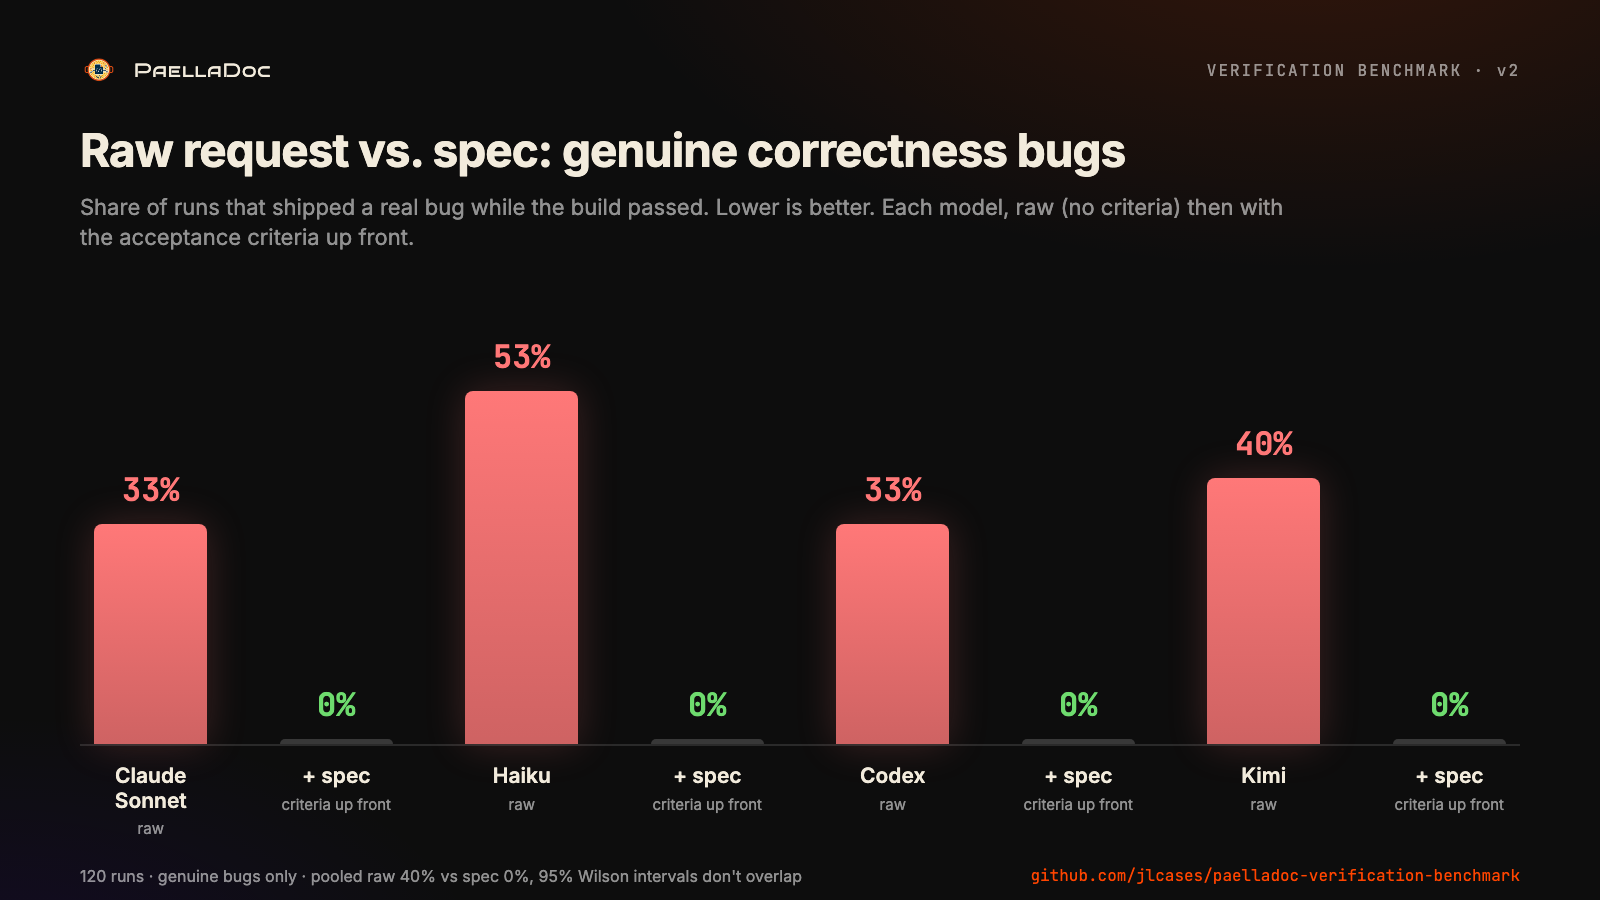
\includegraphics[width=0.92\textwidth]{figures/bug-rate.png}
\caption{Genuine-bug rate per model, raw request versus the same request with acceptance criteria up front. Every model drops to zero genuine bugs with the spec.}
\label{fig:bugrate}
\end{figure}

\subsection{Frontier extension}
The configurations a skeptic would name to dismiss the finding do not close the raw gap on their own (Table~\ref{tab:frontier}, Figure~\ref{fig:frontier}). Claude Opus~4.8 at maximum reasoning effort --- the strongest configuration tested --- still shipped a genuine bug in 13\% of raw runs and produced a fully correct feature in only 67\% of them. On the single hardest feature, both Opus configurations failed 2 of 3 raw runs, and they failed on \emph{different} runs of that feature (one going bug, ok, bug; the other bug, bug, ok). With the criteria up front, every extension configuration reached a 0\% genuine-bug rate and 100\% all-pass rate.

\begin{table}[h]
\centering
\caption{Frontier extension (added after the pre-registration, labeled as such): genuine-bug rate (raw) and all-pass rate (raw), 15 runs per cell. With the spec, all configurations reach 0\% genuine bugs and 100\% all-pass.}
\label{tab:frontier}
\begin{tabular}{lccc}
\toprule
Configuration & genuine-bug (raw) & all-pass (raw) & with spec \\
\midrule
Claude Opus 4.8 (high effort) & 13\% & 53\% & 0\% / 100\% \\
Claude Opus 4.8 (max effort) & 13\% & 67\% & 0\% / 100\% \\
Codex / GPT-5.5 (xhigh effort) & 33\% & 53\% & 0\% / 100\% \\
\bottomrule
\end{tabular}
\end{table}

\begin{figure}[h]
\centering
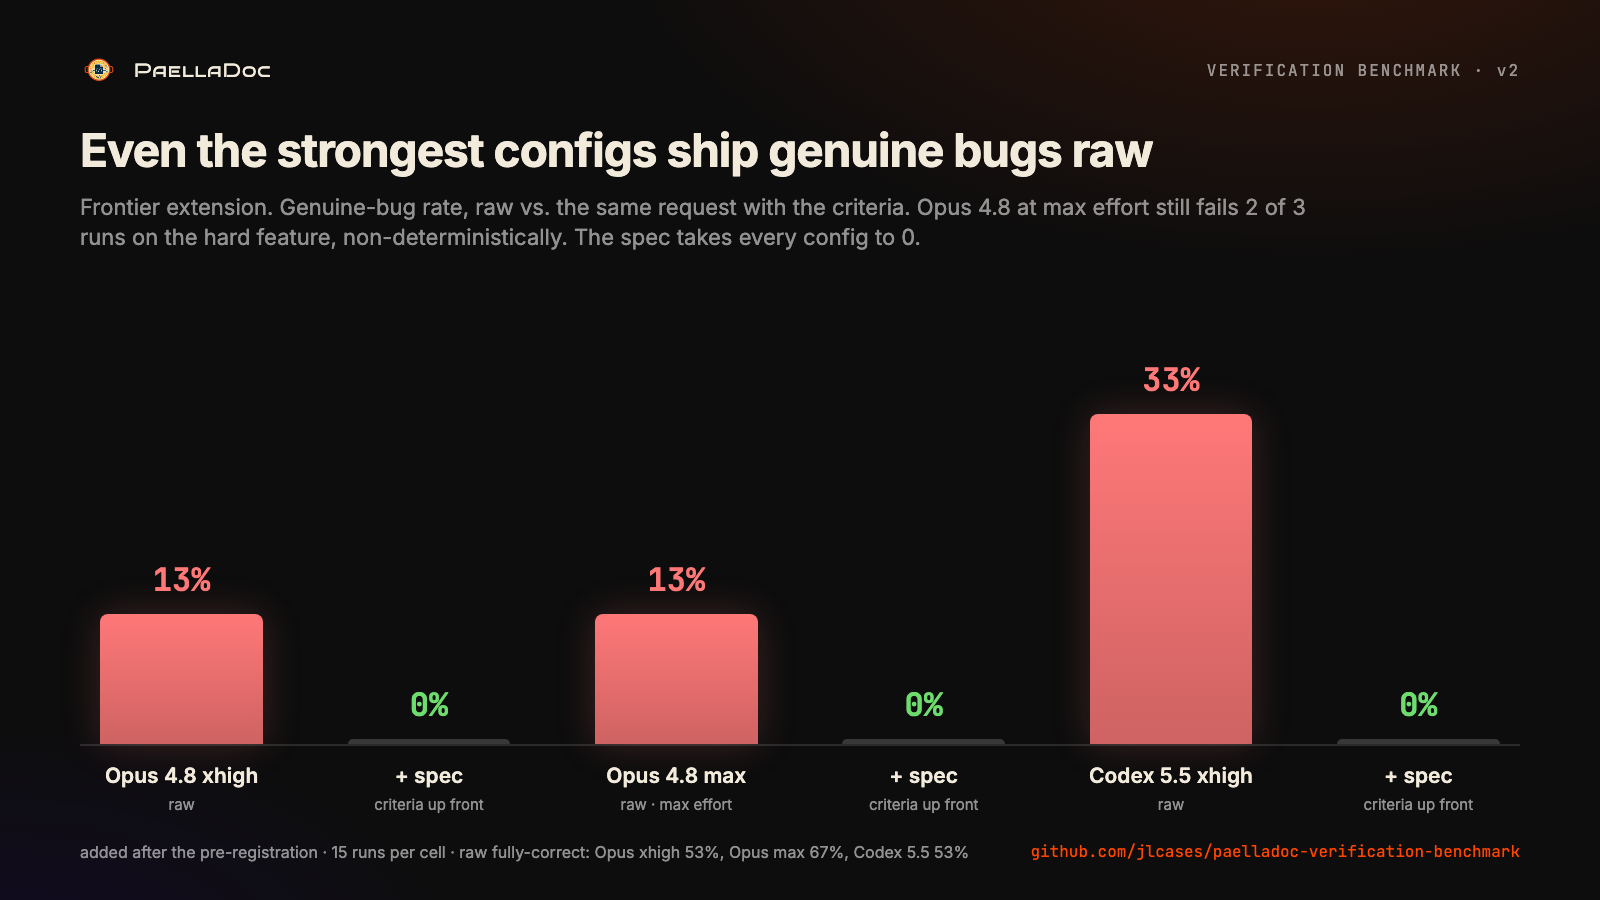
\includegraphics[width=0.92\textwidth]{figures/frontier.png}
\caption{Frontier extension: even the strongest configurations ship genuine bugs in the raw condition; the specification takes every one to zero.}
\label{fig:frontier}
\end{figure}

\subsection{Non-determinism}
Of 70 cells (each three runs), 11 (16\%) disagreed with themselves on the all-criteria-pass outcome, and \emph{every} unstable cell was in the raw condition. The hardest feature was unstable even for both Opus configurations. A single run per cell would have been misleading in roughly one cell in six; the specification removed the instability along with the bugs.

\section{Threats to Validity}

\textbf{Coverage.} Five features, one repository, one stack, one language. The result is directional for ``real AI coding,'' not a universal law; more features and additional stacks are the obvious next work, and we treat the present study as a small, fully-published probe rather than a settled claim.

\textbf{Told $\rightarrow$ passes.} The spec condition is given the criteria the gate then checks. This is mitigated by (a) the independent gate applying the \emph{same} assertions to both conditions, so the raw arm is not held to a softer bar, and (b) the pre-committed \texttt{genuine}/\texttt{contract} split, so the headline counts only failures a competent implementation should avoid without being told. The comparison measures the value of telling the agent the criteria, not a tautology; a held-out-criteria condition (where the gate checks criteria not given to the spec arm) is a natural strengthening we leave to future work.

\textbf{Single-rater tagging.} The \texttt{genuine}/\texttt{contract} tags were assigned by one author before the runs and published; independent multi-rater tagging with an agreement statistic would further harden the primary metric.

\textbf{Model drift.} Hosted models change under fixed names; results are a snapshot. Run-time configurations are recorded with the artifacts.

\section{Discussion}
\label{sec:discussion}

The natural reading of these numbers is ``better models fail less,'' and they do: the raw genuine-bug rate falls from 53\% for the cheapest model to 13\% for the strongest frontier configuration. But it never reaches zero, the failures concentrate on the part that is actually hard, and they are non-deterministic. We therefore think the finding is better read as a statement about trust than about capability.

The question was never whether the model \emph{can} produce correct code. It is whether you can trust that \emph{this} run --- the one in front of you --- is correct, without executing it. On a system where the same model and the same prompt return correct, correct, broken across three runs, the answer is no, and it stays no for the strongest configuration money can buy. What recovers the information is an explicit definition of correct that travels with the change and a gate that executes against it. Coherence, in this sense, is a property of the process, not of the model.

A practical corollary is economic: because the specification, not the model, is the dominant variable for correctness on these tasks, a cheaper model supplied with criteria reaches the correctness of a frontier model without them. Verification decouples cost from trust.

\section{Conclusion}

A green build is not evidence that agent-generated code is correct. Across 210 published runs, a raw request shipped a genuine correctness bug in a large fraction of cases with the build green, the same model flipped between correct and broken on identical prompts, and even a frontier model at maximum reasoning effort did not escape either problem. Writing the acceptance criteria up front and gating ``done'' on execution against them removed the genuine-bug rate entirely and let a cheap model match an expensive one. The study is small and we publish it as such; every diff and verdict is available so the method can be attacked and every number reproduced.

\section*{Reproducibility}
The pre-registered protocol, the five features and their acceptance-criteria tags, the runner, the independent execution-based scorer, all 210 diffs with per-run verdicts, and the results are public at \repo. Because every diff is published, all reported numbers can be re-derived by re-scoring the artifacts without running a single agent. Agent outputs are not bit-reproducible by design (non-determinism is the object of study); what is reproducible is the protocol, the gate, and the published artifacts.

\end{document}
